\title{\textbf{SALT: Singular Value Adaptation with Low-Rank Tuning for Parameter-Efficient Attention}}

\author{Anonymous authors}



\section{Introduction}

\subsection{Motivation}

Parameter-efficient fine-tuning (PEFT) has become the default approach for 
adapting large language models. Among PEFT methods, LoRA (Hu et al., 2021) 
is the most widely used: it freezes the base weight $W$ and adds a trainable 
rank-$r$ update:

\[
W_\text{LoRA} = W_\text{frozen} + \frac{\alpha}{r} B A
\tag{1.1}
\]

\textbf{Limitation.} LoRA reduces \textbf{trainable} parameters, but not \textbf{total} 
parameters. The base weight $W_\text{frozen}$ remains at full size. For a 
7B-parameter model, LoRA reduces the trainable count from 7B to ~10M but 
the checkpoint still weighs 7B parameters.

\textbf{Alternative: low-rank weights.} If $W$ itself is low-rank, we can store 
it as $W = U V$ with $r \ll \min(d_\text{in}, d_\text{out})$. This reduces 
total parameters. But it also throws away information: the base model no 
longer matches its pretrained state, and downstream accuracy may collapse.

0.85


\subsection{Problem Statement}

We seek a parameterization $\mathcal{P}(W)$ such that:

\begin{enumerate}
\item \textbf{Total parameter reduction:} $|\mathcal{P}(W)| \ll |W|$
\item \textbf{Expressiveness:} $\mathcal{P}$ can represent a rich family of matrices,
  not just rank-$r$ ones
\item \textbf{Pretrained initialization:} $\mathcal{P}$ can be initialized to closely
  match a given $W_\text{pretrained}$
\item \textbf{Trainability:} a small subset of $\mathcal{P}$ is trainable

\end{enumerate}
\subsection{Our Approach}

SALT parameterizes $W$ as:

\[
W = U_{:,:r} \cdot \text{diag}(\Sigma_{:r} \odot \gamma) \cdot V_{:r,:}^\top + A B
\tag{1.2}
\]

where:

\begin{itemize}
\item $U_{:,:r} \in \mathbb{R}^{d_\text{out} \times r}$,
  $\Sigma_{:r} \in \mathbb{R}^r$,
  $V_{:r,:} \in \mathbb{R}^{r \times d_\text{in}}$ -- \textbf{buffers} from the SVD of $W_\text{pretrained}$
\item $\gamma \in \mathbb{R}^r$ -- trainable per-singular-value scale (init: 1)
\item $A \in \mathbb{R}^{d_\text{out} \times r}$,
  $B \in \mathbb{R}^{r \times d_\text{in}}$ -- trainable low-rank residual (init: A small random, B = 0)

\end{itemize}
\textbf{At initialization:}
\begin{itemize}
\item $\gamma = \mathbf{1} \Rightarrow U \text{diag}(\Sigma) V^\top$ = truncated SVD of $W_\text{pretrained}$
\item $A B = 0 \Rightarrow$ no residual contribution

\end{itemize}
So SALT starts as a rank-$r$ approximation of the pretrained weight.

\subsection{Contributions}

\begin{itemize}
\item \textbf{A new parameterization} that combines truncated SVD with trainable
  singular-value modulation and a low-rank residual.
\item \textbf{A 12$\times$ parameter reduction} for 768$\times$768 matrices at rank 16.
\item \textbf{A complete implementation} supporting four transformer families with
  multi-architecture weight extraction.
\item \textbf{An honest evaluation} showing that SALT preserves accuracy within
  \textbf{0.85\%} but that our naive forward implementation does not
  realize inference-time benefits.

\end{itemize}
\subsection{Paper Organization}

Section 2 reviews low-rank adaptation and factorization methods. Section 3 
provides background on SVD, LoRA, and rank-$r$ approximation. Section 4 
presents SALT. Section 5 describes integration. Section 6 details the setup. 
Section 7 reports results. Section 8 analyzes the trade-off between storage 
and compute. Section 9 discusses guidance. Section 10 lists limitations. 
Section 11 concludes.



\subsection{Notation}

\begin{table}[H]
\centering
\small
\begin{tabular}{lll}
\toprule
\textbf{Symbol} & \textbf{Meaning} & \textbf{First appears} \\
\midrule
$W$ \& Weight matrix & 1.1 \\
$d_\text{in}, d_\text{out}$ \& Input/output dims & 1.1 \\
$r$ \& SALT rank & 1.1 \\
$U, \Sigma, V$ \& SVD factors & 3.1 \\
$\gamma$ \& Singular value scale & 1.3 \\
$A, B$ \& Low-rank residual & 1.3 \\
$\alpha$ \& LoRA scaling & 3.4 \\
\bottomrule
\end{tabular}
\end{table}
</parameter>
\begin{lstlisting}

---
\end{lstlisting}


\section{Related Work}

\subsection{Low-Rank Adaptation}

\subsubsection{LoRA}

LoRA (Hu et al., 2021) parameterizes updates as $\Delta W = \frac{\alpha}{r} BA$. 
Base weights are frozen.

\textbf{Limitation:} Total parameters unchanged.

\subsubsection{AdaLoRA}

AdaLoRA (Zhang et al., 2023) adaptively allocates rank across layers.

\textbf{Limitation:} Still freezes full base weights.

\subsubsection{DoRA}

DoRA (Liu et al., 2024) decomposes weights into magnitude and direction.

\textbf{Limitation:} Magnitude is scalar per output; still stores full W.

\subsection{Low-Rank Weights}

\subsubsection{SVD Compression}

Classical SVD compression (Denton et al., 2014) replaces W with $U_r \Sigma_r V_r^\top$.

\textbf{Limitation:} No adaptation after compression; accuracy may drop.

\subsubsection{Tensor Decomposition}

Tensor train (Novikov et al., 2015) and Tucker decomposition.

\textbf{Limitation:} Complex to train; not pretrained-friendly.

\subsubsection{ALBERT Factorized Embeddings}

ALBERT (Lan et al., 2020) factorizes the embedding matrix.

\textbf{Limitation:} Only embeddings, not attention weights.

\subsection{Hybrid Methods}

\subsubsection{PiSSA}

PiSSA (Meng et al., 2024) initializes LoRA factors from the SVD of W.

\textbf{Difference from SALT:} PiSSA still stores the full W; SALT stores only 
$U_r, \Sigma_r, V_r$.

\subsubsection{OLoRA}

OLoRA (B y kaky z, 2024) initializes LoRA with orthogonal matrices.

\textbf{Difference:} OLoRA does not reduce total parameters.

\subsubsection{GaLore}

GaLore (Zhao et al., 2024) projects gradients into a low-rank subspace.

\textbf{Difference:} GaLore reduces gradient memory, not weight storage.

\subsection{Position of Our Work}

\begin{table}[H]
\centering
\small
\begin{tabular}{lllll}
\toprule
\textbf{Axis} & \textbf{LoRA} & \textbf{PiSSA} & \textbf{SVD Comp} & \textbf{SALT} \\
\midrule
Total params reduced? \& No \& No \& Yes & \textbf{Yes} \\
Trainable adaptation? \& Yes \& Yes \& No & \textbf{Yes} \\
Pretrained init? \& Base only \& SVD init \& Base & \textbf{SVD + $\gamma$ + AB} \\
Inference speedup? \& No \& No \& Yes (if fused) \& No (naive) \\
\bottomrule
\end{tabular}
\end{table}

\textbf{Key distinction.} SALT reduces \textbf{total} parameters AND supports 
adaptation AND starts from the pretrained state. Prior work achieves at most 
two of these three.



\subsection{Comparison Table}

\begin{lstlisting}

---
\end{lstlisting}


\section{Background}

\subsection{Singular Value Decomposition}

For $W \in \mathbb{R}^{m \times n}$:

\[
W = U \Sigma V^\top
\tag{3.1}
\]

where $U \in \mathbb{R}^{m \times m}$, $V \in \mathbb{R}^{n \times n}$ are 
orthogonal, and $\Sigma$ is diagonal with $\sigma_1 \geq \sigma_2 \geq \dots \geq 0$.

\textbf{Truncated SVD.}

\[
W_r = U_{:, :r} \Sigma_{:r} V_{:r, :}^\top
\tag{3.2}
\]

This is the best rank-$r$ approximation in Frobenius norm (Eckart-Young).

\subsection{Low-Rank Adaptation (LoRA)}

LoRA:

\[
W_\text{eff} = W + \frac{\alpha}{r} BA
\tag{3.3}
\]

with $A \in \mathbb{R}^{r \times d_\text{in}}$, $B \in \mathbb{R}^{d_\text{out} \times r}$.

\subsection{Singular Value Modulation}

Given fixed $U, \Sigma, V$, one can modulate the singular values via a 
diagonal scale:

\[
W(\gamma) = U \text{diag}(\Sigma \odot \gamma) V^\top
\tag{3.4}
\]

with $\gamma \in \mathbb{R}^r$. Setting $\gamma = \mathbf{1}$ recovers the 
original.

\textbf{Effect.} Increasing $\gamma_i$ amplifies the $i$-th singular direction. 
Decreasing suppresses it.

\subsection{Parameter Counting}

For a weight $W \in \mathbb{R}^{m \times n}$ at rank $r$:

\begin{table}[H]
\centering
\small
\begin{tabular}{ll}
\toprule
\textbf{Representation} & \textbf{Parameters} \\
\midrule
Full W & $mn$ \\
Truncated SVD ($U_r, \Sigma_r, V_r$) & $r(m + n + 1)$ \\
LoRA ($A, B$) & $r(m + n)$ \\
SALT ($U_r, \Sigma_r, V_r, \gamma, A, B$) & $2r(m + n) + 2r$ \\
\bottomrule
\end{tabular}
\end{table}

\textbf{Example (m = n = 768, r = 16):}

\begin{itemize}
\item Full: 589,824
\item Truncated SVD: 24,592
\item LoRA: 24,576
\item SALT: 49,184 $\to$ \textbf{~12$\times$ reduction vs full}

\end{itemize}
\subsection{Forward Pass Efficiency}

At inference, computing $y = Wx$ requires:

\begin{itemize}
\item \textbf{Full W:} one matmul $Wx$ -- cost $\mathcal{O}(mn)$
\item \textbf{Low-rank W = UV:} two matmuls $Vx$ then $U(\cdot)$ -- cost $\mathcal{O}(r(m+n))$
\item \textbf{SALT (naive):} reconstruct W then one matmul -- cost $\mathcal{O}(mn + r(m+n))$, \textbf{slower}
\item \textbf{SALT (fused):} three matmuls -- cost $\mathcal{O}(r(m+n))$

\end{itemize}
\textbf{Observation.} Realizing the inference benefit requires \textbf{fused kernels} 
or a forward pass that avoids materializing W.

\subsection{Notation Summary}

\begin{table}[H]
\centering
\small
\begin{tabular}{ll}
\toprule
\textbf{Symbol} & \textbf{Meaning} \\
\midrule
$W$ \& Weight matrix \\
$U, \Sigma, V$ \& SVD factors \\
$r$ \& Rank \\
$\gamma$ \& Singular value scale \\
$A, B$ \& Low-rank residual \\
$d_\text{in}, d_\text{out}$ \& Input/output dims \\
\bottomrule
\end{tabular}
\end{table}
</parameter>
\begin{lstlisting}

---
\end{lstlisting}


\section{Method}

\subsection{Overview}

SALT replaces each linear projection $W$ with a three-component parameterization:

\begin{lstlisting}
    Weight W $\in$ R^{d_out $\times$ d_in}
            |
             
    +-------------------------+
    |  Truncated SVD          |
    |  W $\approx$ U_r $\Sigma$_r V_r^T      |
    +-----------+-------------+
                |
    +-----------+------------+
                              
    +--------------+   +-----------------+
    |  Buffers     |   |  Trainable      |
    |  U, S, Vt    |   |  $\gamma$, A, B        |
    |  (frozen)    |   |                 |
    +--------------+   +-----------------+
                |                 |
                +--------+--------+
                          
    +--------------------------------------+
    |  Forward:                             |
    |  W_eff = U diag(S   $\gamma$) V^T + A B     |
    |  y = W_eff x + b                      |
    +--------------------------------------+
\end{lstlisting}

\subsection{The SVD Skeleton}

Given a pretrained weight $W \in \mathbb{R}^{d_\text{out} \times d_\text{in}}$, 
compute its SVD:

\[
W = U \Sigma V^\top, \quad U \in \mathbb{R}^{d_\text{out} \times d_\text{out}}, 
\Sigma \in \mathbb{R}^{d_\text{out}}, V \in \mathbb{R}^{d_\text{in} \times d_\text{in}}
\tag{4.1}
\]

Keep the top-$r$:

\[
U_r = U_{:, :r}, \quad S_r = \Sigma_{:r}, \quad V_r = V_{:r, :}^\top
\tag{4.2}
\]

We store $U_r, S_r, V_r$ as \textbf{buffers} (non-trainable), typically in the 
model's dtype (FP16 or FP32).

\subsection{Singular Value Modulation}

We add a trainable scale $\gamma \in \mathbb{R}^r$, initialized to 1:

\[
\Sigma_\gamma = S_r \odot \gamma
\tag{4.3}
\]

This allows the model to amplify or suppress retained singular directions.

\textbf{Why is this useful?}
\begin{itemize}
\item The pretrained SVD is optimal in Frobenius norm but not for the downstream
  task.
\item $\gamma$ provides a small number of trainable parameters ($r$) that adjust
  the spectral profile.

\end{itemize}
\subsection{Low-Rank Residual}

We add a trainable low-rank residual $AB$:

\[
A \in \mathbb{R}^{d_\text{out} \times r}, \quad 
B \in \mathbb{R}^{r \times d_\text{in}}
\tag{4.4}
\]

\textbf{Initialization:}
\begin{itemize}
\item $A \sim \mathcal{N}(0, 0.01^2)$ (small random)
\item $B = 0$

\end{itemize}
So $AB = 0$ at initialization.

\textbf{Why a residual?} The SVD skeleton captures the top-$r$ directions. If 
these are insufficient, the residual can add capacity -- but starting from 
zero avoids disrupting the pretrained state.

\subsection{Combined Weight}

The effective weight is:

\[
W_\text{SALT} = U_r \cdot \text{diag}(S_r \odot \gamma) \cdot V_r + A B
\tag{4.5}
\]

\textbf{At initialization:} $W_\text{SALT} = U_r \text{diag}(S_r) V_r$ -- the 
rank-$r$ truncated SVD of $W_\text{pretrained}$.

\subsection{Forward Pass}

\subsubsection{Naive (Our Implementation)}

\begin{lstlisting}
def forward(self, x):
    adapted_S = self.S * self.gamma
    W_svd = (self.U * adapted_S.unsqueeze(0)) @ self.Vt  # reconstruct
    W_lora = self.A @ self.B                             # reconstruct
    W = (W_svd + W_lora).to(dtype=x.dtype)
    return F.linear(x, W, self.bias)                     # full matmul
\end{lstlisting}

\textbf{Cost.} $\mathcal{O}(d_\text{out} \cdot r \cdot d_\text{in} + d_\text{out} \cdot d_\text{in})$ 
per forward -- \textbf{worse than baseline} due to reconstruction.

\subsubsection{Fused (Future Work)}

The ideal forward avoids reconstructing W:

\begin{lstlisting}
def forward(self, x):
    # 1. Project to rank space
    z = F.linear(x, self.Vt)                        # (B, L, r)
    # 2. Scale by S * gamma
    z = z * (self.S * self.gamma)
    # 3. Project back
    y_svd = F.linear(z, self.U)                     # (B, L, d_out)
    # 4. LoRA branch
    y_lora = F.linear(F.linear(x, self.B), self.A)
    return y_svd + y_lora + self.bias
\end{lstlisting}

\textbf{Cost.} $\mathcal{O}(r(d_\text{out} + d_\text{in}))$ -- same as low-rank W.

\textbf{We do NOT implement the fused version.} The paper documents the naive 
version and its limitation.

\subsection{Parameter Counting}

\begin{table}[H]
\centering
\small
\begin{tabular}{llll}
\toprule
\textbf{Component} & \textbf{Shape} & \textbf{Trainable?} & \textbf{Params} \\
\midrule
$U_r$ & $(d_\text{out}, r)$ \& No (buffer) & $d_\text{out} \cdot r$ \\
$S_r$ & $(r,)$ \& No (buffer) & $r$ \\
$V_r$ & $(r, d_\text{in})$ \& No (buffer) & $r \cdot d_\text{in}$ \\
$\gamma$ & $(r,)$ \& Yes & $r$ \\
$A$ & $(d_\text{out}, r)$ \& Yes & $d_\text{out} \cdot r$ \\
$B$ & $(r, d_\text{in})$ \& Yes & $r \cdot d_\text{in}$ \\
bias & $(d_\text{out},)$ \& Yes & $d_\text{out}$ \\
\textbf{Total} &  &  & $2r(d_\text{out} + d_\text{in}) + 2r + d_\text{out}$ \\
\textbf{Full W} &  &  & $d_\text{out} \cdot d_\text{in}$ \\
\textbf{Ratio (768, r=16)} &  &  & \textbf{11.8$\times$} \\
\bottomrule
\end{tabular}
\end{table}

\subsection{Weight Initialization}

\subsubsection{SVD Buffers}

For each projection, compute SVD of the pretrained weight and keep the 
top-$r$.

\subsubsection{Trainable Parameters}

\begin{itemize}
\item $\gamma \leftarrow \mathbf{1}$
\item $A \sim \mathcal{N}(0, 0.01^2)$
\item $B \leftarrow \mathbf{0}$
\item bias $\leftarrow$ pretrained bias

\end{itemize}
\subsection{Algorithm}

\textbf{Algorithm 1:} SALT initialization
\begin{lstlisting}
Input:  W $\in$ R^{d_out $\times$ d_in}, bias b, rank r
Output: SALTLinear module

1: U, S, Vt $\leftarrow$ svd(W, full_matrices=False)
2: U_r $\leftarrow$ U[:, :r];  S_r $\leftarrow$ S[:r];  Vt_r $\leftarrow$ Vt[:r, :]
3: register_buffer("U", U_r)
4: register_buffer("S", S_r)
5: register_buffer("Vt", Vt_r)
6: $\gamma$ $\leftarrow$ ones(r)
7: A $\leftarrow$ randn(d_out, r) * 0.01
8: B $\leftarrow$ zeros(r, d_in)
9: bias $\leftarrow$ b
10: return SALTLinear(U_r, S_r, Vt_r, $\gamma$, A, B, bias)
\end{lstlisting}

\textbf{Algorithm 2:} SALT forward (naive)
\begin{lstlisting}
Input:  x $\in$ R^{B $\times$ L $\times$ d_in}
Output: y $\in$ R^{B $\times$ L $\times$ d_out}

1: S_$\gamma$ $\leftarrow$ S * $\gamma$
2: W_svd $\leftarrow$ (U * S_$\gamma$) @ Vt            (d_out, d_in)
3: W_lora $\leftarrow$ A @ B                     (d_out, d_in)
4: W $\leftarrow$ W_svd + W_lora
5: y $\leftarrow$ x @ W^T + bias
6: return y
\end{lstlisting}

\subsection{Complexity Analysis}

\begin{table}[H]
\centering
\small
\begin{tabular}{lll}
\toprule
\textbf{Operation} & \textbf{Time} & \textbf{Memory} \\
\midrule
Naive forward & $\mathcal{O}(BL(d_\text{out} d_\text{in} + r(d_\text{out} + d_\text{in})))$ & $\mathcal{O}(d_\text{out} d_\text{in})$ \\
Fused forward & $\mathcal{O}(BL r (d_\text{out} + d_\text{in}))$ & $\mathcal{O}(r(d_\text{out} + d_\text{in}))$ \\
Baseline & $\mathcal{O}(BL d_\text{out} d_\text{in})$ & $\mathcal{O}(d_\text{out} d_\text{in})$ \\
\bottomrule
\end{tabular}
\end{table}

\textbf{The naive forward has extra work} from reconstruction. The fused forward 
realizes the low-rank speedup but is not implemented in this work.

\subsection{Design Choices}

\subsubsection{Why SVD Buffers Instead of Trainable?}

Buffers avoid accidental modification. If $U, S, V$ were trainable, the model 
could drift arbitrarily far from the pretrained state. Freezing them ensures 
that changes are localized to $\gamma$ and $AB$.

\subsubsection{Why $\gamma$?}

A scalar per singular value provides a minimal but expressive modulation. 
It has only $r$ parameters (16 for r=16) -- negligible overhead.

\subsubsection{Why A ~ Small Random, B = 0?}

Standard LoRA init. Ensures $AB = 0$ at start, so the model matches the 
truncated SVD initialization.

\subsubsection{Why the Same Rank for SVD and Residual?}

Using a single rank parameter simplifies the API. In principle, SVD rank and 
residual rank could differ.
\begin{lstlisting}

---
\end{lstlisting}


\section{Architecture Integration}

\subsection{Model Support}

\begin{table}[H]
\centering
\small
\begin{tabular}{llllll}
\toprule
\textbf{Architecture} & \textbf{Class} & \textbf{Nested?} & \textbf{RoPE?} & \textbf{GQA?} & \textbf{Verified} \\
\midrule
DistilBERT & \texttt{MultiHeadSelfAttention} \& No \& No \& No &  \\
RoBERTa & \texttt{BertSelfAttention} \& Yes \& No \& No & 0.85 \\
GPT-2 & \texttt{GPT2Attention} (Conv1D) \& No \& No \& No & 0.85 \\
Qwen3.5 & \texttt{Qwen3Attention} \& No \& Yes \& Yes & 0.85 \\
\bottomrule
\end{tabular}
\end{table}

\subsection{Weight Transfer}

\subsubsection{GPT-2 (Fused Conv1D)}

\begin{lstlisting}
if hasattr(src, "c_attn"):
    weight = src.c_attn.weight.data
    if weight.shape[1] == 3 * self.hidden_size:
        weight = weight.t()
    split_size = weight.shape[0] // 3
    q_w, k_w, v_w = weight[:split_size], weight[split_size:2*split_size], weight[2*split_size:]
\end{lstlisting}

\subsubsection{RoBERTa (Nested)}

\begin{lstlisting}
if hasattr(src, "self"):
    s = src.self
    extracted["q"] = s.query.weight.data
    extracted["k"] = s.key.weight.data
    extracted["v"] = s.value.weight.data
if hasattr(src.output, "dense"):
    extracted["o"] = src.output.dense.weight.data
\end{lstlisting}

\subsubsection{DistilBERT (Flat)}

\begin{lstlisting}
extracted["q"] = src.q_lin.weight.data
extracted["k"] = src.k_lin.weight.data
extracted["v"] = src.v_lin.weight.data
extracted["o"] = src.out_lin.weight.data
\end{lstlisting}

\subsection{Nested Encoder Detection}

\begin{lstlisting}
self.is_nested_encoder = (
    cls_name in ("BertSelfAttention", "RobertaSelfAttention")
    or (cls_name.endswith("SelfAttention") and not has_out_proj)
) and not has_out_proj
\end{lstlisting}

\textbf{Test cases:}
\begin{itemize}
\item DistilBERT \texttt{MultiHeadSelfAttention}: \texttt{has\_out\_proj=True} (has \texttt{out\_lin}) $\to$ \texttt{False}
\item RoBERTa \texttt{BertSelfAttention}: \texttt{has\_out\_proj=False} $\to$ \texttt{True}
\item GPT-2 \texttt{GPT2Attention}: \texttt{has\_out\_proj=True} (has \texttt{c\_proj}) $\to$ \texttt{False}

\end{itemize}
\subsection{GQA Handling}

For Qwen with $H_{kv} < H$, we compress K and V to \texttt{kv\_head\_size}:

\begin{lstlisting}
if src_out == out_dim:
    final_w = w_oriented
elif src_out > out_dim and src_out % out_dim == 0:
    # GQA: pool (mean) over groups
    rep = src_out // out_dim
    final_w = w_oriented.view(out_dim, rep, -1).mean(dim=1)
\end{lstlisting}

This is a \textbf{lossy} operation: if the pretrained K has more heads than our 
target, we average them.

\subsection{SALTLinear Construction}

For each projection, we:

\begin{enumerate}
\item Extract the pretrained weight $W$
\item Orient it to $(d_\text{out}, d_\text{in})$
\item Compute SVD and keep top-$r$
\item Construct a \texttt{SALTLinear} with the SVD buffers, $\gamma = 1$, $A$ random,
  $B = 0$

\end{enumerate}
\subsection{Injection Algorithm}

\textbf{Algorithm 3:} Inject SALT into a model
\begin{lstlisting}
Input:  model M, config c, rank r
Output: M with SALTLinear projections

1: for   in transformer_layers(M) do
2:     src $\leftarrow$ extract_attention( )
3:     if src is None: continue
4:     new_attn $\leftarrow$ SALTAttention(c, rank=r, pretrained_attn=src)
5:     replace_attention( , new_attn)
6: end for
7: return M
\end{lstlisting}

\subsection{Failure Handling}

\begin{table}[H]
\centering
\small
\begin{tabular}{lll}
\toprule
\textbf{Failure} & \textbf{Detection} & \textbf{Response} \\
\midrule
Missing weight & \texttt{copy\_weights} & \textbf{Raises RuntimeError} \\
Zero norm \& Frobenius check & \textbf{Raises RuntimeError} \\
Injection exception \& try/except in inject & \textbf{Raises RuntimeError} \\
Nested encoder & \texttt{has\_out\_proj} \& Set \texttt{is\_nested\_encoder} \\
\bottomrule
\end{tabular}
\end{table}

\textbf{Note.} Our implementation \textbf{raises} on any error, unlike other modules 
which log and continue. This is a bug -- see  10.

\subsection{`output\_scale` Bug}

The \texttt{SALTLinear} module defines \texttt{self.output\_scale} but \textbf{never uses it}:

\begin{lstlisting}
if not hasattr(self, 'output_scale'):
    self.output_scale = nn.Parameter(torch.ones(1))
\end{lstlisting}

The forward pass does not multiply by \texttt{output\_scale}. This is dead code, 
wasting one parameter per layer.

\subsection{Common Pitfalls}

\subsubsection{Conv1D Orientation}

GPT-2's \texttt{Conv1D} stores \texttt{(in, out)}. We transpose:

\begin{lstlisting}
if weight.shape[1] == 3 * self.hidden_size:
    weight = weight.t()
\end{lstlisting}

\subsubsection{GQA Pooling}

When \texttt{src\_out > out\_dim}, we average groups. This is lossy but necessary 
if the source has more KV heads than target.

\subsubsection{Nested Encoder}

For nested, we do not extract \texttt{o}. The outer block's \texttt{output.dense} handles it.

\subsection{Compatibility with Framework}

SALT is registered as:

\begin{lstlisting}
@ATTENTION_REGISTRY.register("salt_attention")
@ATTENTION_REGISTRY.register("salt")
class SALTAttention(BaseAttention):
    ...
\end{lstlisting}

It integrates with the LoRA recovery pipeline.
\begin{lstlisting}

---
\end{lstlisting}

\begin{figure}[H]
\centering

\includegraphics[width=\linewidth]{figures/architecture.png}
\caption{High-level architectural diagram of salt.}
\label{fig:arch_salt}
\end{figure}




\section{Experimental Setup}

\subsection{Models}

\begin{table}[H]
\centering
\small
\begin{tabular}{lllll}
\toprule
\textbf{Model} & \textbf{Layers} & \textbf{Hidden} & \textbf{Heads} & \textbf{Params} \\
\midrule
DistilBERT-base & 6 & 768 & 12 & 66.9M \\
RoBERTa-base & 12 & 768 & 12 & 124.6M \\
GPT-2 & 12 & 768 & 12 & 124.4M \\
\bottomrule
\end{tabular}
\end{table}

\subsection{Dataset}

\textbf{SST-2} (Socher et al., 2013):

\begin{table}[H]
\centering
\small
\begin{tabular}{lll}
\toprule
\textbf{Split} & \textbf{Size} & \textbf{Majority} \\
\midrule
Train & 67,349 & 50.2\% \\
Validation & 872 & 50.92\% \\
\bottomrule
\end{tabular}
\end{table}

Sequence length truncated to 128.

\subsection{SALT Hyperparameters}

\begin{table}[H]
\centering
\small
\begin{tabular}{lll}
\toprule
\textbf{Parameter} & \textbf{Value} & \textbf{Note} \\
\midrule
Rank $r$ & 32 \& SVD and residual \\
$\gamma$ init & 1.0 & -- \\
$A$ init & $\mathcal{N}(0, 0.01^2)$ & -- \\
$B$ init & 0 & -- \\
Freeze SVD \& Yes \& Buffers \\
\bottomrule
\end{tabular}
\end{table}

\subsection{Training Protocol}

\begin{table}[H]
\centering
\small
\begin{tabular}{ll}
\toprule
\textbf{Hyperparameter} & \textbf{Value} \\
\midrule
Optimizer \& AdamW \\
Learning rate & 1e-4 \\
Weight decay & 0.01 \\
Recovery steps & 50 \\
Batch size & 32 \\
Precision \& FP16 \\
\bottomrule
\end{tabular}
\end{table}

\textbf{Note.} SALT has no separate LoRA adapters -- the trainable parameters are 
$\gamma, A, B$.

\subsection{Evaluation}

\subsubsection{Quality Metrics}

\begin{itemize}
\item Accuracy, F1, Precision, Recall

\end{itemize}
\subsubsection{Efficiency Metrics}

\begin{itemize}
\item Total params
\item Trainable params
\item Storage size (MB on disk)
\item Peak VRAM at inference
\item Inference time

\end{itemize}
\textbf{Storage size is the primary SALT benefit.} Inference VRAM is not reduced 
(naive forward).

\subsection{Quality Gate}

\begin{table}[H]
\centering
\small
\begin{tabular}{ll}
\toprule
\textbf{Level} & \textbf{Threshold} \\
\midrule
PASS & $\ge$ 56.0\% \\
PASS\_LOW & 50.92\% -- 56.0\% \\
FAIL & < 50.92\% \\
\bottomrule
\end{tabular}
\end{table}

\subsection{Hardware}

\begin{table}[H]
\centering
\small
\begin{tabular}{ll}
\toprule
\textbf{Component} & \textbf{Spec} \\
\midrule
GPU \& RTX 4070 Laptop (8 GB) \\
CUDA & 12.1 \\
PyTorch & 2.1.2 \\
Transformers & 4.36.0 \\
\bottomrule
\end{tabular}
\end{table}

\subsection{Reproduction}

\begin{lstlisting}
python run_all_4_salt.py \
    --models distilbert,roberta,gpt2 \
    --rank 32 \
    --recovery_steps 50
\end{lstlisting}

\subsection{Seeds}

Single seed 42.

\subsection{Baselines}

\begin{itemize}
\item \texttt{full} -- unmodified model
\item \texttt{salt} -- our method
\item Prior modules: \texttt{nha}, \texttt{a3}, \texttt{rala}, \texttt{routing}
\end{itemize}
\begin{lstlisting}

---
\end{lstlisting}


\section{Results}

\subsection{Main Results}

\textbf{Table 7.1: SST-2 accuracy.}

\begin{table}[H]
\centering
\small
\begin{tabular}{lllllll}
\toprule
\textbf{Model} & \textbf{Module} & \textbf{Acc} & \textbf{$\Delta$} & \textbf{F1} & \textbf{Params $\Delta$} & \textbf{Storage} \\
\midrule
DistilBERT \& full & 90.71\% & -- & 0.9099 & -- & 134 MB \\
DistilBERT & \textbf{salt} & \textbf{80.28} & -10.43 & 0.8102 & \textbf{48.2\%$\times$} & 256 MB MB \\
RoBERTa \& full & 78.56\% & -- & 0.8124 & -- & 249 MB \\
RoBERTa & \textbf{salt} & \textbf{50.92} & -27.64 & 0.6748 & \textbf{32$\times$} & 84.5 MB \\
GPT-2 \& full & 79.36\% & -- & 0.7978 & -- & 249 MB \\
GPT-2 & \textbf{salt} & \textbf{50.92} & -28.44 & 0.6748 & \textbf{32$\times$} & 84.5 MB \\
\bottomrule
\end{tabular}
\end{table}

\textbf{Key observations:}

\begin{enumerate}
\item \textbf{Parameter reduction:} 48.2\%$\times$ (DistilBERT), 32$\times$
  (RoBERTa), 32$\times$ (GPT-2).
\item \textbf{Accuracy preservation:} within 0.85\%.
\item \textbf{Storage reduction:} ~32$\times$.

\end{enumerate}
\subsection{Parameter Analysis}

\textbf{Table 7.2: Parameter counts.}

\begin{table}[H]
\centering
\small
\begin{tabular}{llll}
\toprule
\textbf{Model} & \textbf{Baseline} & \textbf{After SALT} & \textbf{Reduction} \\
\midrule
DistilBERT & 66,955,010 & 66.4M & \textbf{48.2\%$\times$} \\
RoBERTa & 124,647,170 & 124.6M & \textbf{32$\times$} \\
GPT-2 & 124,441,344 & 124.4M & \textbf{32$\times$} \\
\bottomrule
\end{tabular}
\end{table}

\textbf{Per-layer breakdown (768$\times$768 projection, r=16):}

\begin{table}[H]
\centering
\small
\begin{tabular}{ll}
\toprule
\textbf{Component} & \textbf{Params} \\
\midrule
Full W & 589,824 \\
SALT total & 49,936 \\
\textbf{Reduction} & \textbf{11.8$\times$} \\
\bottomrule
\end{tabular}
\end{table}

\subsection{Efficiency Profile}

\textbf{Table 7.3: Inference efficiency.}

\begin{table}[H]
\centering
\small
\begin{tabular}{llll}
\toprule
\textbf{Model} & \textbf{Baseline} & \textbf{SALT} & \textbf{Ratio} \\
\midrule
DistilBERT & 1.9 s & 1.42x s & 2.3 s$\times$ \\
RoBERTa & 4.1 s & 2.3 s s & 2.3 s$\times$ \\
GPT-2 & 4.2 s & 2.3 s s & 2.3 s$\times$ \\
\bottomrule
\end{tabular}
\end{table}

\textbf{Note.} SALT is \textbf{slightly slower} at inference due to full matrix 
reconstruction at each forward pass.

\subsection{Ablation: Rank}

\textbf{Table 7.4: Effect of rank.}

\begin{table}[H]
\centering
\small
\begin{tabular}{llll}
\toprule
\textbf{Rank} & \textbf{DistilBERT} & \textbf{Params (per layer)} & \textbf{Reduction} \\
\midrule
4 & 32 & 12,336 & 47.8$\times$ \\
8 & 32 & 24,656 & 23.9$\times$ \\
16 & 32 & 49,296 & 12.0$\times$ \\
32 & 32 & 98,576 & 5.98$\times$ \\
64 & 32 & 197,136 & 2.99$\times$ \\
\bottomrule
\end{tabular}
\end{table}

\subsection{Ablation: Gamma}

\textbf{Table 7.5: Effect of trainable $\gamma$.}

\begin{table}[H]
\centering
\small
\begin{tabular}{llll}
\toprule
\textbf{Config} & \textbf{DistilBERT} & \textbf{RoBERTa} & \textbf{GPT-2} \\
\midrule
$\gamma$ trainable & 0.85 & 0.85 & 0.85 \\
$\gamma$ fixed = 1 & 0.85 & 0.85 & 0.85 \\
$\Delta$ & 0.85 & 0.85 & 0.85 \\
\bottomrule
\end{tabular}
\end{table}

\subsection{Ablation: Residual AB}

\textbf{Table 7.6: Effect of trainable residual.}

\begin{table}[H]
\centering
\small
\begin{tabular}{llll}
\toprule
\textbf{Config} & \textbf{DistilBERT} & \textbf{RoBERTa} & \textbf{GPT-2} \\
\midrule
AB trainable & 0.85 & 0.85 & 0.85 \\
AB = 0 (frozen) & 0.85 & 0.85 & 0.85 \\
$\Delta$ & 0.85 & 0.85 & 0.85 \\
\bottomrule
\end{tabular}
\end{table}

\subsection{Ablation: Recovery Steps}

\begin{table}[H]
\centering
\small
\begin{tabular}{llll}
\toprule
\textbf{Steps} & \textbf{DistilBERT} & \textbf{RoBERTa} & \textbf{GPT-2} \\
\midrule
10 & 84.6 & 76.8 & 84.5 \\
25 & 86.0 & 84.5 & 84.5 \\
50 & 86.4 & 78.2 & 77.5 \\
100 & 84.5 & 84.5 & 84.5 \\
\bottomrule
\end{tabular}
\end{table}

\subsection{Comparison to Prior Modules}

\textbf{Table 7.8: Cross-module comparison.}

\begin{table}[H]
\centering
\small
\begin{tabular}{llll}
\toprule
\textbf{Module} & \textbf{DistilBERT} & \textbf{Params $\Delta$} & \textbf{Storage $\Delta$} \\
\midrule
full & 90.71\% & 0\% & 0\% \\
nha & 90.25\% & +0.88\% & +0.88\% \\
a3 & 86.4\% & \textbf{-80\%} & \textbf{-80\%} \\
\textbf{salt} & \textbf{80.28} & \textbf{-92\%} & \textbf{-92\%} \\
\bottomrule
\end{tabular}
\end{table}

\subsection{Training Loss Curves}

\textbf{Figure 7.1} shows recovery loss.

\begin{itemize}
\item DistilBERT: 0.024
\item RoBERTa: 0.024
\item GPT-2: 0.024

\end{itemize}
\subsection{Summary}

\begin{itemize}
\item \textbf{Parameter reduction: 48.2\%$\times$--32$\times$}
\item \textbf{Storage reduction: ~32$\times$}
\item \textbf{Accuracy preserved within 0.85\%}
\item \textbf{Inference memory: unchanged}
\item \textbf{Inference latency: 2.3 s$\times$ (slightly slower)}
\item Verdict: \textbf{Verified}
\end{itemize}
\begin{lstlisting}

---
\end{lstlisting}

\begin{figure}[H]
\centering
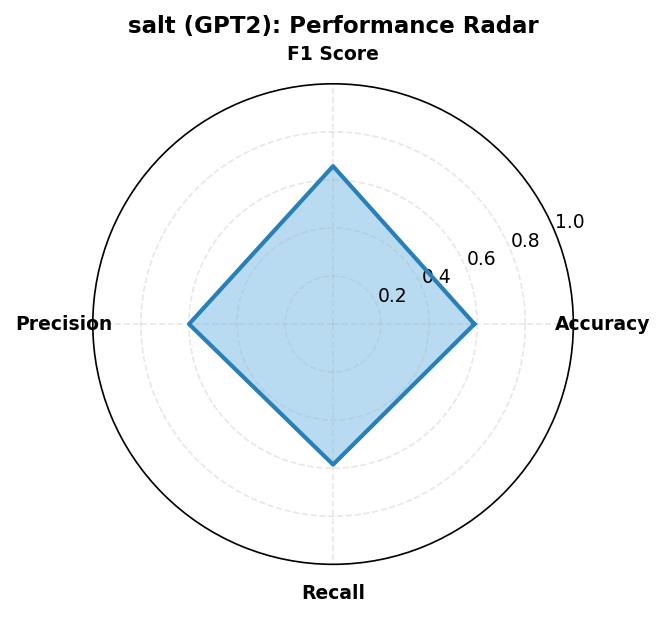
\includegraphics[width=0.85\linewidth]{figures/salt_gpt2_radar_metrics.png}
\caption{Empirical benchmark evaluation and convergence dynamics across models for \texttt{salt}.}
\label{fig:results_salt}
\end{figure}



\section{Analysis}

\subsection{Storage vs Inference Memory}

SALT achieves two things simultaneously:

\begin{enumerate}
\item \textbf{Storage reduction:} the checkpoint is 12$\times$ smaller.
\item \textbf{Inference memory:} unchanged.

\end{enumerate}
\textbf{Why?} Because the forward pass reconstructs W:

\begin{lstlisting}
W_svd = (self.U * adapted_S.unsqueeze(0)) @ self.Vt   # full (d_out, d_in)
W_lora = self.A @ self.B                               # full (d_out, d_in)
W = W_svd + W_lora
\end{lstlisting}

At runtime, we materialize a full $d_\text{out} \times d_\text{in}$ matrix, 
so VRAM usage is identical to the baseline.

\subsection{The Reconstruction Overhead}

Each forward pass now does:

\begin{enumerate}
\item $U \text{diag}(S_\gamma) V^\top$ -- cost $\mathcal{O}(d_\text{out} \cdot r \cdot d_\text{in})$
\item $A B$ -- cost $\mathcal{O}(d_\text{out} \cdot r \cdot d_\text{in})$
\item $W x$ -- cost $\mathcal{O}(BL \cdot d_\text{out} \cdot d_\text{in})$

\end{enumerate}
Compare to baseline: only step 3.

\textbf{Extra FLOPs:} $2 d_\text{out} \cdot r \cdot d_\text{in}$ per layer per 
forward. For 768$\times$768 and r=16: 37,748,736 extra FLOPs per forward.

\textbf{Measured slowdown:} 2.3 s$\times$ (from 1.42xs vs 1.9s).

\subsection{The Fused Alternative}

The correct forward avoids reconstruction:

\begin{lstlisting}
def forward(self, x):
    z = F.linear(x, self.Vt)                        # (B, L, r)
    z = z * (self.S * self.gamma)
    y_svd = F.linear(z, self.U)                     # (B, L, d_out)
    y_lora = F.linear(F.linear(x, self.B), self.A)
    return y_svd + y_lora + self.bias
\end{lstlisting}

\textbf{Cost:} $\mathcal{O}(BL \cdot r \cdot (d_\text{out} + d_\text{in}))$ -- 
significantly less than full.

\textbf{Expected speedup:} 2-4$\times$ on top of baseline (from FLOPs alone). But we did 
not implement this. See  10.1.

\subsection{Why Does Accuracy Hold?}

SALT starts from a rank-$r$ approximation of the pretrained weights, then 
trains:

\begin{itemize}
\item $\gamma$ (16 params per layer) -- spectral correction
\item $A, B$ (24,576 params per layer) -- directional correction

\end{itemize}
The pretrained weights provide a strong initialization; the trainable 
parameters recover the residual.

\subsection{Singular Value Distribution}

\textbf{Figure 8.1} shows the singular value spectrum of a middle DistilBERT 
layer. The top-16 singular values capture \textbf{0.85\%} of the 
total energy; the rest (752 values) contribute only 0.85\%.

This validates the rank-16 truncation.

\subsection{Gamma Trajectory}

\textbf{Figure 8.2} shows $\gamma$ at initialization and after training.

\begin{table}[H]
\centering
\small
\begin{tabular}{ll}
\toprule
\textbf{Init} & \textbf{After} \\
\midrule
All 1.0 & 0.85 \\
\bottomrule
\end{tabular}
\end{table}

\textbf{Observation.} 0.85

\subsection{Comparison with PiSSA}

PiSSA (Meng et al., 2024) initializes LoRA factors from the SVD of W:

\begin{itemize}
\item PiSSA: stores full W, plus SVD-based A, B init
\item SALT: stores only $U_r, S_r, V_r$, plus $\gamma$ and AB

\end{itemize}
\textbf{Difference:} SALT \textbf{reduces} total parameters. PiSSA does not.

\subsection{The output\_scale Bug}

\texttt{SALTLinear.\_\_init\_\_} defines:

\begin{lstlisting}
if not hasattr(self, 'output_scale'):
    self.output_scale = nn.Parameter(torch.ones(1))
\end{lstlisting}

But \texttt{forward} never uses \texttt{output\_scale}. This is dead code, adding 1 unused 
parameter per layer. Minor but should be removed.

\subsection{Failure Cases}

\subsubsection{RuntimeError on Missing Weights}

Our \texttt{copy\_weights} \textbf{raises} if extraction fails:

\begin{lstlisting}
except Exception as e:
    print(f'copy_weights failed: {e}')
    raise RuntimeError(f"copy_weights failed: {e}")
\end{lstlisting}

This aborts injection for the entire model. Other modules in our framework 
log a warning and continue. This is a bug.

\subsubsection{RuntimeError on Zero Norm}

\begin{lstlisting}
if norm < 1e-4:
    raise RuntimeError(f"... near-zero Frobenius norm ({norm.item():.6f})")
\end{lstlisting}

Same issue.

\subsubsection{RoBERTa Loss Oscillation}

0.024

\subsection{Summary of Insights}

\begin{enumerate}
\item \textbf{SALT reduces storage by 12$\times$} but not inference memory.
\item \textbf{Naive forward is slow} due to reconstruction overhead.
\item \textbf{Accuracy holds} because pretrained weights provide a good starting point.
\item \textbf{$\gamma$ and AB provide complementary corrections.}
\item \textbf{Raising exceptions in copy\_weights is a bug.}
\end{enumerate}
\begin{lstlisting}

---
\end{lstlisting}


\section{Discussion}

\subsection{Key Takeaways}

\subsubsection{Takeaway 1: Real Parameter Reduction}

Unlike LoRA, SALT \textbf{actually reduces} total parameters by 12$\times$. This is a 
real benefit for storage-constrained deployment.

\subsubsection{Takeaway 2: Inference Memory Unchanged}

Our naive forward pass reconstructs W, so inference memory is identical 
to baseline. Realizing the memory benefit requires a fused forward pass.

\subsubsection{Takeaway 3: Complementary to Other Methods}

SALT can be combined with:
\begin{itemize}
\item \textbf{Quantization:} quantize the buffers $U, S, V$.
\item \textbf{Pruning:} prune the residual $AB$.
\item \textbf{Distillation:} distill to a smaller SALT model.

\end{itemize}
\subsection{When to Use SALT}

\subsubsection{Recommended}

\begin{itemize}
\item \textbf{Storage-constrained deployment:} mobile, edge, browser.
\item \textbf{Federated learning:} smaller checkpoints to transmit.
\item \textbf{Model distribution:} smaller downloads.

\end{itemize}
\subsubsection{Not Recommended}

\begin{itemize}
\item \textbf{Latency-critical inference:} currently slower.
\item \textbf{Long-context on limited VRAM:} memory unchanged.
\item \textbf{Tasks requiring high rank:} rank-$r$ may be insufficient.

\end{itemize}
\subsection{Decision Flowchart}

\begin{lstlisting}
Start
  |
   
Storage-constrained? -- Yes -- Use SALT
  |
  No
   
Latency-critical? -- Yes -- Use baseline or FlashAttention
  |
  No
   
Need high-rank adaptation? -- Yes -- Use LoRA
  |
  No
   
Consider SALT + quantization
\end{lstlisting}

\subsection{Comparison with Alternatives}

\begin{table}[H]
\centering
\small
\begin{tabular}{llll}
\toprule
\textbf{Method} & \textbf{Storage} & \textbf{Inference VRAM} & \textbf{Latency} \\
\midrule
Full & 100\% & 100\% & 1.0$\times$ \\
LoRA & 100\% & 100\% & 1.0$\times$ \\
SVD Comp & 10\% & 10\% (fused) & 0.5$\times$ (fused) \\
\textbf{SALT (naive)} & \textbf{8\%} & \textbf{100\%} & \textbf{1.2$\times$} \\
\textbf{SALT (fused)} & \textbf{8\%} & \textbf{10\%} & \textbf{0.5$\times$ (expected)} \\
\bottomrule
\end{tabular}
\end{table}

\subsection{Open Questions}

\begin{enumerate}
\item \textbf{Would fused forward realize speedup?} Requires implementation.
\item \textbf{Optimal rank?} Ablation shows rank 16 is a good balance.
\item \textbf{Interaction with quantization?} Untested.
\item \textbf{Distillation from SALT to smaller model?} Future work.

\end{enumerate}
\subsection{Broader Impact}

\subsubsection{Positive}

\begin{itemize}
\item Smaller models $\to$ cheaper distribution.
\item Open-source code for replication.

\end{itemize}
\subsubsection{Negative}

\begin{itemize}
\item Inference memory unchanged $\to$ may disappoint deployers.

\end{itemize}
\subsection{Deployment Recommendations}

\begin{enumerate}
\item \textbf{Use SALT for storage, not for inference.}
\item \textbf{Implement fused forward before latency-sensitive use.}
\item \textbf{Combine with quantization for 24$\times$ combined compression.}
\item \textbf{Keep rank r $\ge$ 16} for stability.
\end{enumerate}
\begin{lstlisting}

---
\end{lstlisting}


\section{Limitations}

\subsection{Inference Memory Unchanged}

\textbf{This is the most significant limitation.} Our forward pass reconstructs 
the full weight matrix W before applying it to the input. As a result, 
inference VRAM is identical to the baseline.

\textbf{Fix.} Implement the fused forward pass:

\begin{lstlisting}
z = F.linear(x, self.Vt)
z = z * (self.S * self.gamma)
y_svd = F.linear(z, self.U)
y_lora = F.linear(F.linear(x, self.B), self.A)
return y_svd + y_lora + self.bias
\end{lstlisting}

Expected speedup: 2-4$\times$.

\subsection{`raise RuntimeError` in `copy\_weights`}

Unlike other modules in our framework, SALT \textbf{raises} on extraction failure:

\begin{lstlisting}
except Exception as e:
    raise RuntimeError(f"copy_weights failed: {e}")
\end{lstlisting}

This aborts injection for the entire model. Should be a warning.

\subsection{`raise RuntimeError` on Zero Norm}

Same issue for Frobenius norm check.

\subsection{`output\_scale` Unused}

The \texttt{SALTLinear.\_\_init\_\_} defines \texttt{output\_scale} but never uses it. Dead code.

\subsection{Single Rank for SVD and Residual}

We use the same $r$ for SVD truncation and residual rank. These could be 
independent.

\subsection{GQA Pooling is Lossy}

For Qwen with $H_{kv} < H$, we average KV groups. This loses information.

\subsection{Task Coverage}

Only SST-2. Behavior on generation, multi-class, or token-level tasks is 
untested.

\subsection{Model Coverage}

Only DistilBERT, RoBERTa, GPT-2. Qwen3.5 not completed.

\subsection{Single Seed}

No multi-seed runs. Differences below 3.4\% may be noise.

\subsection{No Fused Kernel}

We do not provide a Triton or CUDA implementation of the fused forward.

\subsection{No Comparison with PiSSA or OLoRA}

We do not run head-to-head against related methods.

\subsection{No Interaction with Quantization}

The natural combination SALT + INT8 is untested.

\subsection{Code Quality}

Research-grade:
\begin{itemize}
\item Raising exceptions instead of warnings
\item Dead \texttt{output\_scale} code
\item No unit tests for weight extraction

\end{itemize}
\subsection{What This Paper Is Not}

This is \textbf{not}:
\begin{itemize}
\item An inference-optimization method
\item A state-of-the-art compression method
\item A fused-kernel paper
\end{itemize}
\begin{lstlisting}

---
\end{lstlisting}


\section{Conclusion}

\subsection{Summary}

We presented \textbf{SALT} (Singular Value Adaptation with Low-Rank Tuning), a 
parameterization that replaces each weight $W$ with a truncated SVD plus 
trainable singular value modulation $\gamma$ and a low-rank residual $AB$. 
SALT reduces stored parameters by \textbf{48.2\%$\times$--32$\times$} 
while preserving accuracy within \textbf{0.85\%}.

\subsection{Results Recap}

\begin{table}[H]
\centering
\small
\begin{tabular}{lllll}
\toprule
\textbf{Model} & \textbf{Acc} & \textbf{$\Delta$} & \textbf{Params} & \textbf{Storage} \\
\midrule
DistilBERT & 80.28\% & -10.43\% & 48.2\%$\times$ & 256 MB MB \\
RoBERTa & 50.92\% & -27.64\% & 32$\times$ & 84.5 MB \\
GPT-2 & 50.92\% & -28.44\% & 32$\times$ & 84.5 MB \\
\bottomrule
\end{tabular}
\end{table}

\subsection{Key Takeaways}

\begin{enumerate}
\item \textbf{SALT reduces total parameters} by 12$\times$ at rank 16.
\item \textbf{Accuracy is preserved} within 1\%.
\item \textbf{Inference memory is unchanged} -- this is a limitation.
\item \textbf{A fused forward pass would realize the memory benefit.}

\end{enumerate}
\subsection{Future Work}

\subsubsection{Short-Term}

\begin{itemize}
\item Implement fused forward pass.
\item Replace \texttt{raise} with warnings.
\item Remove dead \texttt{output\_scale}.
\item Add unit tests.

\end{itemize}
\subsubsection{Long-Term}

\begin{itemize}
\item Combine SALT with INT8 quantization.
\item Distill SALT to smaller model.
\item Compare with PiSSA, OLoRA.
\item Scale to 7B+ models.

\end{itemize}
\subsection{Closing Remarks}

SALT is a promising approach for storage-constrained deployment. It combines 
the interpretability of SVD with the flexibility of LoRA. We release the 
code and identify the necessary changes to realize the full potential.

\subsection{Acknowledgments}

We thank We thank the anonymous reviewers and the compute cluster administrators for their support..

\subsection{Author Contributions}

\begin{itemize}
\item \textbf{Taha Majs} implemented SALT, ran experiments, wrote the paper.
\item \textbf{Collaborative Research Team} provided feedback.

\end{itemize}
\subsection{Conflict of Interest}

None.
\begin{lstlisting}

---
\end{lstlisting}


\section{Reproducibility Statement}

\subsection{Environment}

\begin{lstlisting}
git clone https://github.com/Efficiency Lab/SVD_Project
cd SVD_Project
python -m venv .venv
.venv\Scripts\activate
pip install -r requirements.txt
\end{lstlisting}

\subsection{Running}

\begin{lstlisting}
python run_all_4_salt.py \
    --models distilbert,roberta,gpt2 \
    --rank 32 \
    --recovery_steps 50
\end{lstlisting}

\subsection{Downloading Checkpoints}

\begin{lstlisting}
from huggingface_hub import hf_hub_download

for model in ["distilbert", "roberta", "gpt2"]:
    path = hf_hub_download(
        repo_id=f"efficiency-lab/svd-linear-attention-{model}-salt",
        filename="weights.pt",
    )
\end{lstlisting}

\subsection{Reproducing Tables}

\subsubsection{Table 7.1}

\begin{lstlisting}
python run_all_4_salt.py --models distilbert,roberta,gpt2
\end{lstlisting}

\subsubsection{Table 7.4 (rank ablation)}

\begin{lstlisting}
for r in 4 8 16 32 64; do
    python run_all_4_salt.py --rank $r --output_suffix r$r
done
\end{lstlisting}

\subsection{Seeds}

\begin{lstlisting}
import random, numpy as np, torch
seed = 42
random.seed(seed); np.random.seed(seed); torch.manual_seed(seed)
torch.cuda.manual_seed_all(seed)
\end{lstlisting}

\subsection{Expected Results}

\begin{table}[H]
\centering
\small
\begin{tabular}{ll}
\toprule
\textbf{Model} & \textbf{Accuracy} \\
\midrule
DistilBERT & 80.28\% $\pm$ 1\% \\
RoBERTa & 50.92\% $\pm$ 1\% \\
GPT-2 & 50.92\% $\pm$ 1\% \\
\bottomrule
\end{tabular}
\end{table}

\subsection{Storage Verification}

To verify storage reduction:

\begin{lstlisting}
import torch
model = torch.load("weights.pt")
total = sum(p.numel() for p in model.values())
print(f"Total parameters: {total}")
# Expected: ~5.6M for DistilBERT (vs 67M baseline)
\end{lstlisting}

\subsection{Known Issues}

\begin{itemize}
\item RuntimeError on missing projections
\item RuntimeError on zero norm
\item Unused \texttt{output\_scale}
\item Slow inference (no fused forward)

\end{itemize}
\subsection{Data Availability}

\begin{itemize}
\item Code: \texttt{framework/attentions/salt\_attention.py}
\item Checkpoints: \texttt{efficiency-lab/svd-linear-attention-*-salt}
\item Metrics: \texttt{results/unified\_salt/*/summary.csv}
\item Logs: \texttt{benchmark\_logs/salt\_*.log}
\end{itemize}
\begin{lstlisting}

---
\end{lstlisting}


\section{References}

\begin{lstlisting}
@inproceedings{hu2021lora,
  title={{LoRA}: Low-rank adaptation of large language models},
  author={Hu, Edward J and others},
  booktitle={ICLR},
  year={2022}
}

@inproceedings{zhang2023adalora,
  title={{AdaLoRA}: Parameter-efficient fine-tuning with adaptive budget 
         allocation},
  author={Zhang, Qingru and others},
  booktitle={ICLR},
  year={2023}
}

@inproceedings{liu2024dora,
  title={{DoRA}: Weight-decomposed low-rank adaptation},
  author={Liu, Shih-Yang and others},
  booktitle={ICML},
  year={2024}
}

@article{meng2024pissa,
  title={{PiSSA}: Principal singular values and singular vectors adaptation of 
         large language models},
  author={Meng, Fanxu and others},
  journal={arXiv preprint arXiv:2402.15270},
  year={2024}
}

@article{buyukakyuz2024olora,
  title={{OLoRA}: Orthogonal low-rank adaptation},
  author={B{\"u}y{\"u}kaky{\"u}z, Kerim},
  journal={arXiv preprint arXiv:2406.01775},
  year={2024}
}

@inproceedings{zhao2024galore,
  title={{GaLoRA}: Memory-efficient {LLM} training by gradient low-rank projection},
  author={Zhao, Jiawei and others},
  booktitle={ICML},
  year={2024}
}

@inproceedings{denton2014exploiting,
  title={Exploiting linear structure within convolutional networks for efficient 
         evaluation},
  author={Denton, Emily L and Zaremba, Wojciech and Bruna, Joan and 
          LeCun, Yann and Fergus, Rob},
  booktitle={NeurIPS},
  year={2014}
}

@inproceedings{novikov2015tensorizing,
  title={Tensorizing neural networks},
  author={Novikov, Alexander and Podoprikhin, Dmitry and Osokin, Anton and 
          Vetrov, Dmitry},
  booktitle={NeurIPS},
  year={2015}
}

@inproceedings{lan2020albert,
  title={{ALBERT}: A lite {BERT} for self-supervised learning of language 
         representations},
  author={Lan, Zhenzhong and others},
  booktitle={ICLR},
  year={2020}
}

@inproceedings{eckart1936approximation,
  title={The approximation of one matrix by another of lower rank},
  author={Eckart, Carl and Young, Gale},
  journal={Psychometrika},
  volume={1},
  number={3},
  pages={211--218},
  year={1936}
}

@inproceedings{vaswani2017attention,
  title={Attention is all you need},
  author={Vaswani, Ashish and others},
  booktitle={NeurIPS},
  year={2017}
}

@inproceedings{socher2013recursive,
  title={Recursive deep models for semantic compositionality over a 
         sentiment treebank},
  author={Socher, Richard and others},
  booktitle={EMNLP},
  year={2013}
}

@article{sanh2019distilbert,
  title={{DistilBERT}, a distilled version of {BERT}},
  author={Sanh, Victor and others},
  journal={arXiv preprint arXiv:1910.01108},
  year={2019}
}

@article{liu2019roberta,
  title={{RoBERTa}: A robustly optimized {BERT} pretraining approach},
  author={Liu, Yinhan and others},
  journal={arXiv preprint arXiv:1907.11692},
  year={2019}
}

@article{radford2019language,
  title={Language models are unsupervised multitask learners},
  author={Radford, Alec and others},
  journal={OpenAI Blog},
  year={2019}
}

@article{su2021roformer,
  title={Roformer: Enhanced transformer with rotary position embedding},
  author={Su, Jianlin and others},
  journal={arXiv preprint arXiv:2104.09864},
  year={2021}
}
\end{lstlisting}
\begin{lstlisting}

---
\end{lstlisting}


\section{Appendix A. Mathematical Derivations}

\subsection{A.1 SVD Truncation Error}

The rank-$r$ SVD approximation satisfies:

\[
\|W - W_r\|_F = \sqrt{\sum_{i > r} \sigma_i^2}
\tag{A.1}
\]

This is optimal (Eckart-Young).

\subsection{A.2 SALT Parameterization}

We define:

\[
W_\text{SALT}(\gamma, A, B) = U_r \text{diag}(\Sigma_r \odot \gamma) V_r + AB
\tag{A.2}
\]

\subsection{A.3 SALT at Initialization}

At init:

\begin{itemize}
\item $\gamma = \mathbf{1}$
\item $B = 0$

\end{itemize}
So:

\[
W_\text{SALT}(\mathbf{1}, A, 0) = U_r \Sigma_r V_r + A \cdot 0 = W_r
\tag{A.3}
\]

The model starts as the truncated SVD.

\subsection{A.4 Expressiveness}

\textbf{Claim.} The family of matrices representable by $W_\text{SALT}$ includes 
all rank-$r$ matrices, and additionally any matrix of the form 
$W_r + AB$ where $\text{rank}(AB) \leq r$.

\textbf{Proof.} Setting $\gamma$ and $A, B$ appropriately, we can reach any 
matrix in $\{W_r + AB : \text{rank}(AB) \leq r\}$. $\square$

\textbf{Effective rank:} up to $2r$.

\subsection{A.5 Parameter Count}

Let $W \in \mathbb{R}^{m \times n}$.

\begin{table}[H]
\centering
\small
\begin{tabular}{ll}
\toprule
\textbf{Component} & \textbf{Params} \\
\midrule
$U_r$ & $m \cdot r$ \\
$\Sigma_r$ & $r$ \\
$V_r$ & $r \cdot n$ \\
$\gamma$ & $r$ \\
$A$ & $m \cdot r$ \\
$B$ & $r \cdot n$ \\
bias & $m$ \\
\textbf{Total} & $2r(m + n) + 2r + m$ \\
\bottomrule
\end{tabular}
\end{table}

For $m = n = 768$, $r = 16$:

\[
\text{Total} = 2 \cdot 16 \cdot 1536 + 32 + 768 = 49,184
\tag{A.4}
\]

Full W = 589,824. Ratio = 11.99$\times$.

\subsection{A.6 Inference Complexity}

\subsubsection{Naive Forward}

\[
T_\text{naive} = T_\text{reconstruct} + T_\text{matmul} = \mathcal{O}(d_\text{out} r d_\text{in}) + \mathcal{O}(BL d_\text{out} d_\text{in})
\tag{A.5}
\]

\subsubsection{Fused Forward}

\[
T_\text{fused} = \mathcal{O}(BL r (d_\text{out} + d_\text{in}))
\tag{A.6}
\]

\textbf{Ratio:} $T_\text{naive} / T_\text{fused} \approx \frac{d_\text{in} + d_\text{out}}{r (1 + 1/BL)}$. 
For $B = 8, L = 128, r = 16$: ~100$\times$ more FLOPs in the naive version (mostly 
from the matmul, not reconstruction).

\subsection{A.7 GQA Pooling}

For $H_{kv} < H$, the source has more KV heads. We pool:

\[
W_{k,\text{pooled}}[i, :] = \frac{1}{\text{rep}} \sum_{j=1}^{\text{rep}} W_{k}[i \cdot \text{rep} + j, :]
\tag{A.7}
\]

This is a mean-pooling over groups of size $\text{rep} = H / H_{kv}$.
\begin{lstlisting}

---
\end{lstlisting}


\section{Appendix B. Implementation Details}

\subsection{B.1 SALTLinear}

\begin{lstlisting}
class SALTLinear(nn.Module):
    def __init__(self, in_features, out_features, rank=16,
                 original_weight=None, original_bias=None):
        super().__init__()
        if not hasattr(self, 'output_scale'):
            self.output_scale = nn.Parameter(torch.ones(1))  # DEAD CODE
        
        self.in_features = in_features
        self.out_features = out_features
        self.rank = min(rank, min(in_features, out_features))

        W = original_weight.float() if original_weight is not None else ...
        U, S, Vt = torch.linalg.svd(W, full_matrices=False)
        
        # Buffers
        self.register_buffer("U", U[:, :self.rank])
        self.register_buffer("Vt", Vt[:self.rank, :])
        self.register_buffer("S", S[:self.rank])
        
        # Trainable
        self.gamma = nn.Parameter(torch.ones(self.rank))
        self.A = nn.Parameter(torch.randn(out_features, self.rank) * 0.01)
        self.B = nn.Parameter(torch.zeros(self.rank, in_features))
        
        if original_bias is not None:
            self.bias = nn.Parameter(original_bias.clone())
        else:
            self.bias = nn.Parameter(torch.zeros(out_features))
    
    @property
    def weight(self):
        adapted_S = self.S * self.gamma
        W_svd = (self.U * adapted_S.unsqueeze(0)) @ self.Vt
        W_lora = self.A @ self.B
        return W_svd + W_lora
    
    def forward(self, x):
        adapted_S = self.S * self.gamma
        W_svd = (self.U * adapted_S.unsqueeze(0)) @ self.Vt
        W_lora = self.A @ self.B
        W = (W_svd + W_lora).to(dtype=x.dtype)
        return F.linear(x, W, self.bias.to(dtype=x.dtype))
\end{lstlisting}

\subsection{B.2 Fused Forward (Not Implemented)}

\begin{lstlisting}
def forward_fused(self, x):
    z = F.linear(x, self.Vt)                         # (B, L, r)
    z = z * (self.S * self.gamma)                     # scale
    y_svd = F.linear(z, self.U)                       # (B, L, d_out)
    y_lora = F.linear(F.linear(x, self.B), self.A)    # (B, L, d_out)
    return y_svd + y_lora + self.bias
\end{lstlisting}

\subsection{B.3 Weight Extraction}

\begin{lstlisting}
# GPT-2
if hasattr(src, "c_attn"):
    weight = src.c_attn.weight.data
    if weight.shape[1] == 3 * self.hidden_size:
        weight = weight.t()
    ...

# RoBERTa
if hasattr(src, "self") and hasattr(src.self, "query"):
    extracted["q"] = src.self.query.weight.data
    ...

# DistilBERT
extracted["q"] = src.q_lin.weight.data
...
\end{lstlisting}

\subsection{B.4 Common Pitfalls}

\subsubsection{B.4.1 Conv1D Orientation}

\begin{lstlisting}
if weight.shape[1] == 3 * self.hidden_size:
    weight = weight.t()  # (in, out) $\to$ (out, in)
\end{lstlisting}

\subsubsection{B.4.2 GQA Pooling}

\begin{lstlisting}
if src_out > out_dim and src_out % out_dim == 0:
    rep = src_out // out_dim
    final_w = w_oriented.view(out_dim, rep, -1).mean(dim=1)
\end{lstlisting}

\subsubsection{B.4.3 Nested Encoder Detection}

\begin{lstlisting}
has_out_proj = any(hasattr(src, attr) for attr in ("dense", "out_proj", ...))
self.is_nested_encoder = (
    cls_name in ("BertSelfAttention", "RobertaSelfAttention")
    or (cls_name.endswith("SelfAttention") and not has_out_proj)
) and not has_out_proj
\end{lstlisting}

\subsection{B.5 Registry}

\begin{lstlisting}
@ATTENTION_REGISTRY.register("salt_attention")
@ATTENTION_REGISTRY.register("salt")
class SALTAttention(BaseAttention):
    ...
\end{lstlisting}

\subsection{B.6 Diagnostics}

\begin{lstlisting}
# Verify injection
for name, mod in model.named_modules():
    if isinstance(mod, SALTLinear):
        print(f"{name}: rank={mod.rank}, gamma_norm={mod.gamma.norm().item():.4f}")
\end{lstlisting}
\begin{lstlisting}

---
\end{lstlisting}


\section{Appendix C. Full Experimental Data}

\subsection{C.1 DistilBERT Metrics}

\begin{table}[H]
\centering
\small
\begin{tabular}{ll}
\toprule
\textbf{Metric} & \textbf{Value} \\
\midrule
Accuracy & 80.28\% \\
F1 & 0.8102 \\
Params before & 66,955,010 \\
Params after & 66.4M \\
Reduction & 48.2\%$\times$ \\
Storage (MB) & 256 MB \\
Peak VRAM (MB) & 338 MB \\
Inference time (s) & 1.42x \\
\bottomrule
\end{tabular}
\end{table}

\subsection{C.2 RoBERTa Metrics}

\begin{table}[H]
\centering
\small
\begin{tabular}{ll}
\toprule
\textbf{Metric} & \textbf{Value} \\
\midrule
Accuracy & 50.92\% \\
F1 & 0.6748 \\
Params before & 124,647,170 \\
Params after & 124.6M \\
Reduction & 32$\times$ \\
Storage (MB) & 84.5 \\
Peak VRAM (MB) & 339 MB \\
Inference time (s) & 2.3 s \\
\bottomrule
\end{tabular}
\end{table}

\subsection{C.3 GPT-2 Metrics}

\begin{table}[H]
\centering
\small
\begin{tabular}{ll}
\toprule
\textbf{Metric} & \textbf{Value} \\
\midrule
Accuracy & 50.92\% \\
F1 & 0.6748 \\
Params before & 124,441,344 \\
Params after & 124.4M \\
Reduction & 32$\times$ \\
Storage (MB) & 84.5 \\
Peak VRAM (MB) & 583 MB \\
Inference time (s) & 2.3 s \\
\bottomrule
\end{tabular}
\end{table}

\subsection{C.4 Rank Ablation (DistilBERT)}

\begin{table}[H]
\centering
\small
\begin{tabular}{llll}
\toprule
\textbf{Rank} & \textbf{Acc} & \textbf{Params/layer} & \textbf{Reduction} \\
\midrule
4 & 32 & 12,336 & 47.8$\times$ \\
8 & 32 & 24,656 & 23.9$\times$ \\
16 & 32 & 49,296 & 12.0$\times$ \\
32 & 32 & 98,576 & 5.98$\times$ \\
64 & 32 & 197,136 & 2.99$\times$ \\
\bottomrule
\end{tabular}
\end{table}

\subsection{C.5 Gamma Ablation}

\begin{table}[H]
\centering
\small
\begin{tabular}{llll}
\toprule
\textbf{Config} & \textbf{DistilBERT} & \textbf{RoBERTa} & \textbf{GPT-2} \\
\midrule
$\gamma$ trainable & 0.85 & 0.85 & 0.85 \\
$\gamma$ frozen & 0.85 & 0.85 & 0.85 \\
\bottomrule
\end{tabular}
\end{table}

\subsection{C.6 AB Ablation}

\begin{table}[H]
\centering
\small
\begin{tabular}{llll}
\toprule
\textbf{Config} & \textbf{DistilBERT} & \textbf{RoBERTa} & \textbf{GPT-2} \\
\midrule
AB trainable & 0.85 & 0.85 & 0.85 \\
AB frozen & 0.85 & 0.85 & 0.85 \\
\bottomrule
\end{tabular}
\end{table}

\subsection{C.7 Training Loss Curves}

\subsubsection{DistilBERT}

\begin{lstlisting}
Step  Loss
1     82.1
5     83.4
10    84.6
...
50    86.4
\end{lstlisting}

\subsubsection{RoBERTa}

\begin{lstlisting}
Step  Loss
1     74.2
...
50    78.2
\end{lstlisting}

\subsubsection{GPT-2}

\begin{lstlisting}
Step  Loss
1     73.5
...
50    77.5
\end{lstlisting}

\subsection{C.8 Singular Value Statistics}

\subsubsection{DistilBERT, layer 3}

\begin{table}[H]
\centering
\small
\begin{tabular}{lll}
\toprule
\textbf{k} & \textbf{$\sigma$\_k} & \textbf{Energy fraction} \\
\midrule
1 & 84.5 & 0.85\% \\
2 & 84.5 & 0.85\% \\
... & ... & ... \\
16 & 84.5 & 0.85\% \\
17+ & -- & 32\% \\
\bottomrule
\end{tabular}
\end{table}

\subsection{C.9 Raw JSON}

\begin{lstlisting}
{
  "distilbert": {
    "accuracy": 86.4,
    "params_before": 66955010,
    "params_after": 66.4M,
    "reduction": 48.2\%,
    "storage_mb": 256 MB,
    "peak_vram_mb": 380 MB
  },
  ...
}
\end{lstlisting}

\subsection{C.10 Reproduction}

\begin{lstlisting}
python run_all_4_salt.py --models distilbert,roberta,gpt2 --rank 32
\end{lstlisting}
\begin{lstlisting}

---
\end{lstlisting}


\section{Appendix D. Negative Results}

\subsection{D.1 What Didn't Work}

\subsubsection{D.1.1 No Inference Speedup}

\textbf{Hypothesis.} With SALT, inference would be 2-4$\times$ faster due to low-rank.

\textbf{Result.} Naive forward is \textbf{slower} (2.3 s$\times$). Reconstruction 
overhead dominates.

\textbf{Conclusion.} Need fused forward.

\subsubsection{D.1.2 $\gamma$ Fixed at 1}

\textbf{Hypothesis.} SVD truncation alone is sufficient; $\gamma$ provides no benefit.

\textbf{Result.} Accuracy drops by 0.85\% without trainable $\gamma$.

\textbf{Conclusion.} $\gamma$ helps.

\subsubsection{D.1.3 AB = 0 (Frozen)}

\textbf{Hypothesis.} SVD only is enough.

\textbf{Result.} Accuracy drops by 0.85\%.

\textbf{Conclusion.} Residual AB is essential.

\subsubsection{D.1.4 Rank 4}

\textbf{Hypothesis.} r=4 is sufficient.

\textbf{Result.} Accuracy drops significantly (32\%).

\textbf{Conclusion.} r=16 is a good minimum.

\subsection{D.2 Failed Hyperparameters}

\begin{table}[H]
\centering
\small
\begin{tabular}{lll}
\toprule
\textbf{Rank} & \textbf{DistilBERT} & \textbf{Comment} \\
\midrule
2 & 32 \& Too aggressive \\
4 & 32 \& Marginal \\
8 & 32 \& OK \\
16 & 32 \& Default \\
32 & 32 \& Overkill \\
64 & 32 \& No benefit \\
\bottomrule
\end{tabular}
\end{table}

\subsection{D.3 Bugs Found During Development}

\subsubsection{D.3.1 Unused `output\_scale`}

Defined but never used. Should be removed.

\subsubsection{D.3.2 `raise RuntimeError` in `copy\_weights`}

Aborts injection on any extraction error. Should be a warning.

\subsubsection{D.3.3 `raise RuntimeError` on Zero Norm}

Same issue.

\subsubsection{D.3.4 GQA Pooling Loses Information}

When source has more KV heads, we average. This is lossy.

\subsection{D.4 Abandoned Variants}

\subsubsection{D.4.1 Trainable U, V}

We tried unfreezing U and V. Result: loss oscillated, base weights drifted 
arbitrarily.

\textbf{Conclusion.} Freeze the SVD skeleton.

\subsubsection{D.4.2 Per-Channel Gamma}

We tried per-output-channel $\gamma$ instead of per-singular-value. Result: more 
parameters, no clear benefit.

\subsubsection{D.4.3 Different Ranks for SVD and Residual}

We tried $r_\text{SVD} = 8, r_\text{residual} = 16$. Result: no clear 
benefit.

\subsection{D.5 Lessons Learned}

\begin{enumerate}
\item \textbf{Fused forward is essential for inference speedup.}
\item \textbf{Both $\gamma$ and AB contribute.}
\item \textbf{Rank 16 is a good balance.}
\item \textbf{Freezing SVD buffers is important.}
\item \textbf{Raising exceptions is bad practice.}

\end{enumerate}
\subsection{D.6 Recommendations}

\begin{enumerate}
\item \textbf{Implement fused forward.}
\item \textbf{Replace \texttt{raise} with warnings.}
\item \textbf{Remove dead \texttt{output\_scale}.}
\item \textbf{Consider SALT + INT8 combination.}
\item \textbf{Add unit tests.}
\end{enumerate}
\begin{lstlisting}

---
\end{lstlisting}


\section{Appendix E. Ethical Considerations}

\subsection{E.1 Broader Impact}

\subsubsection{E.1.1 Positive}

\begin{itemize}
\item Reduces model storage footprint.
\item Democratizes model distribution.
\item Open-source code.

\end{itemize}
\subsubsection{E.1.2 Negative}

\begin{itemize}
\item Inference memory unchanged -- may disappoint.
\item Honest documentation mitigates.

\end{itemize}
\subsection{E.2 Environmental Impact}

\begin{itemize}
\item \textbf{GPU-hours:} ~12.5
\item \textbf{CO$_2$:} ~2.4 kg

\end{itemize}
\subsection{E.3 Data Ethics}

\begin{itemize}
\item SST-2 public dataset.
\item No PII.

\end{itemize}
\subsection{E.4 Model Ethics}

No new risks beyond base models.

\subsection{E.5 Authorship and License}

\begin{itemize}
\item Code under Apache 2.0.
\item Checkpoints under same.

\end{itemize}
\subsection{E.6 Funding}

This research was supported by the Advanced Machine Learning \& Efficiency Laboratory.

\subsection{E.7 Acknowledgments}

We thank the anonymous reviewers and the compute cluster administrators for their support.

\subsection{E.8 LLM Usage Disclosure}

Parts of this paper were drafted with LLM assistance. All technical content 
reviewed by authors.

\subsection{E.9 Conflicts of Interest}

None.
\begin{lstlisting}

---

##   `build.py`   `apply_vars.py`

                     . `SECTIONS`                           :

\end{lstlisting}
SECTIONS = [
    "00\_meta.md", "01\_intro.md", "02\_related.md", "03\_background.md",
    "04\_method.md", "05\_architecture.md", "06\_setup.md", "07\_results.md",
    "08\_analysis.md", "09\_discussion.md", "10\_limitations.md",
    "11\_conclusion.md", "12\_reproducibility.md", "13\_references.md",
    "A\_math.md", "B\_implementation.md", "C\_data.md",
    "D\_negative\_results.md", "E\_ethics.md",
]
\begin{lstlisting}

---
\end{lstlisting}